\documentclass{standalone}
\usepackage{tikz}
\usepackage{mathtools}
\usetikzlibrary{shapes,snakes}


\tikzset{frame/.style = {rectangle, draw=black!90, thick, minimum width=2cm,
    minimum  height = 0.5cm},
  txBeam/.style = {above = 0.8cm, right = 0.8cm},
  rxBeam/.style = {above = 0.8cm, left = 1cm},
  index/.style= {below = 0.5cm}}

\begin{document}
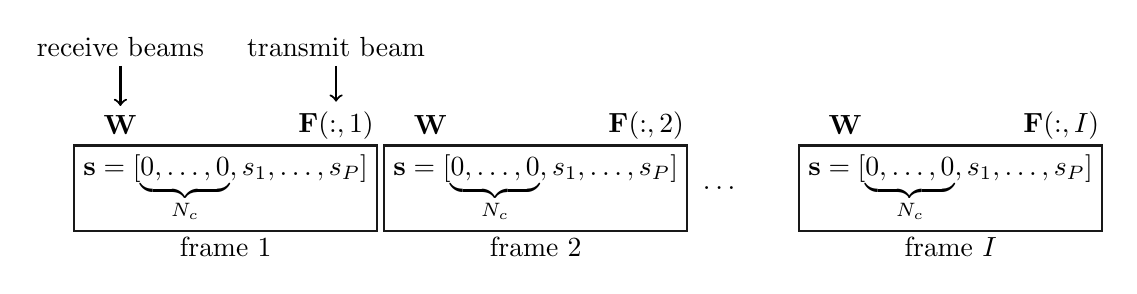
\begin{tikzpicture}
  \node (ref) at (0,0) {};
%  \draw (ref) rectangle ++(2,1) node [anchor = south east]    {\tiny{$\mathbf{F}(:,1)$}};

  \node[frame] (frame1) at (ref) {{$\mathbf{s} = [\underbrace{0, \ldots, 0}_{N_c}, s_1, \ldots, s_P]$}};

  \node[frame] (frame2) [right of = frame1, right =1cm] {{$\mathbf{s} = [\underbrace{0, \ldots, 0}_{N_c}, s_1, \ldots, s_P]$}};

  \node (dots) [right of =frame2, right =1cm] {$\ldots$};

  \node[frame] (frame3) [right of = dots, right = 0.001cm] {{$\mathbf{s} = [\underbrace{0, \ldots, 0}_{N_c}, s_1, \ldots, s_P]$}};

  \node (txBeam1) at (frame1) [txBeam] {{$\mathbf{F}(:,1)$}};
  \node (rxBeam1) at (frame1) [rxBeam] {{$\mathbf{W}$}};
  \node (fIndex1)  at (frame1)  [index]  {{frame 1}};

  \node (txBeam2) at (frame2) [txBeam] {{$\mathbf{F}(:,2)$}};
  \node (rxBeam2) at (frame2) [rxBeam] {{$\mathbf{W}$}};
  \node (fIndex2)  at (frame2)  [index]  {{frame 2}};

  \node (txBeam3) at (frame3) [txBeam] {{$\mathbf{F}(:,I)$}};
  \node (rxBeam3) at (frame3) [rxBeam] {{$\mathbf{W}$}};
  \node (fIndex3)  at (frame3)  [index]  {{frame $I$}};

  \node (txBeamDef) [above of = txBeam1] {transmit beam};
  \node (rxBeamDef) [above of = rxBeam1] {receive beams};

  \draw[->,thick] (txBeamDef) -- (txBeam1);
  \draw[->,thick] (rxBeamDef) -- (rxBeam1);
    
\end{tikzpicture}
\end{document}



%%% Local Variables:
%%% mode: latex
%%% TeX-master: t
%%% End:
